\section{Bayesian Networks}
All probabilistic inference and learning methods are based on the repeated application of basic rules of probability theory.
However, as the number of random variables increases, the complexity of representing and manipulating probability distributions grows exponentially.
Probabilistic graphical models provide a convenient framework to represent and manipulate complex probability distributions.
\\\\Bayesian Networks (BNs) are a formalism to represent probabilistic relationships among a set of random variables.
They allow to:
\begin{itemize}
    \item Visualize the structure of a probabilistic model;
    \item Discover properties of the model (e.g., conditional independencies);
    \item Efficiently perform probabilistic inference and learning, using the structure of the graph;
    \item Represent multiple distrubutions with the same graph, independently of their qualitative aspects
    (e.g., discrete vs continuous variables).
\end{itemize}

\subsection{Bayesian Networks structure}
A Bayesian Network (BN) structure $\mathcal{G}$ is a directed acyclic graph (DAG) where:
\begin{itemize}
    \item Each node represents a random variable;
    \item Each directed edge represent a direct dependency between the two connected variables;
\end{itemize}
It's important to note that the absence of an edge between two nodes doesn't imply independence.
\\\\The given structure $\mathcal{G}$ of a BN encodes these independence assumptions:
\[ \mathcal{I}_l(\mathcal{G}) = \{ \forall i\; \boldsymbol{x}_i \perp \text{NonDescendants}_{\boldsymbol{x}_i} | \text{Parents}_{\boldsymbol{x}_i} \} \]
Each variable $\boldsymbol{x}_i$ is independent of its non-descendants given its parents. 

\begin{figure}[H]
\centering
    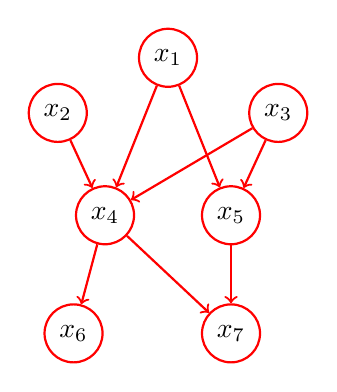
\begin{tikzpicture}[
        node/.style={circle, draw=red, thick, minimum size=18pt},
        arrow/.style={->, red, thick}
    ]
    % Nodes
    \node[node] (x1) at (0, 3.5) {$x_1$};
    \node[node] (x2) at (-1.4, 2.8) {$x_2$};
    \node[node] (x3) at (1.4, 2.8) {$x_3$};
    \node[node] (x4) at (-0.8, 1.5) {$x_4$};
    \node[node] (x5) at (0.8, 1.5) {$x_5$};
    \node[node] (x6) at (-1.2, 0) {$x_6$};
    \node[node] (x7) at (0.8, 0) {$x_7$};
    % Edges
    \draw[arrow] (x1) -- (x4);
    \draw[arrow] (x1) -- (x5);
    \draw[arrow] (x2) -- (x4);
    \draw[arrow] (x3) -- (x4);
    \draw[arrow] (x3) -- (x5);
    \draw[arrow] (x4) -- (x6);
    \draw[arrow] (x4) -- (x7);
    \draw[arrow] (x5) -- (x7);
    \end{tikzpicture}
    \caption{Example of Bayesian Network}
\end{figure}
\subsubsection{Independency Map}
\defib{Independency Map}{
    \begin{itemize}
        \item Let $p$ be a distribution over a set of random variables $\boldsymbol{X}$;
        \item Let $\mathcal{I}(p)$ be the set of independencies that hold in $p$;
    \end{itemize}
    We say that $\mathcal{G}$ is an \textbf{Independency Map} (I-map) for $p$ if $p$ satisfies
    the local independencies encoded in $\mathcal{G}$:
    \[ \mathcal{I}_l(\mathcal{G}) \subseteq \mathcal{I}(p) \]
}
This means that all independencies encoded in the graph $\mathcal{G}$ hold in the distribution $p$.
There can be additional independencies in $p$ that are not encoded in $\mathcal{G}$.

\subsubsection{Factorization}
We say that a distribution $p$ \textbf{factorizes} according to a BN structure $\mathcal{G}$ if $p$ can be expressed as:
\[ p(\boldsymbol{x}_1, \boldsymbol{x}_2, \ldots, \boldsymbol{x}_m) = \prod_{i=1}^{m} p(\boldsymbol{x}_i | \text{Parents}_{\boldsymbol{x}_i}) \]
We have that $\mathcal{G}$ is an I-map for $p$ if and only if $p$ factorizes according to $\mathcal{G}$.
\begin{comment}
%#TODO: Add proof here
\begin{proof}
\end{proof}
\end{comment}

\subsection{Bayesian Network definition}
A Bayesian Network (BN) is a pair $\mathcal{B} = (\mathcal{G}, \mathcal{P})$, where:
\begin{itemize}
    \item $\mathcal{G}$ is a directed acyclic graph (DAG) representing the structure of the BN;
    \item $\mathcal{P}$ is a set of conditional probability distributions (CPDs) associated with the nodes in the graph.
\end{itemize}
$P$ must factorize according to $\mathcal{G}$:
\[ P(\boldsymbol{x}_1, \boldsymbol{x}_2, \ldots, \boldsymbol{x}_m) = \prod_{i=1}^{m} P(\boldsymbol{x}_i | \text{Parents}_{\boldsymbol{x}_i}) \]

\paragraph{Example:}
Consider the following BN structure:
\begin{figure}[H]
\centering
    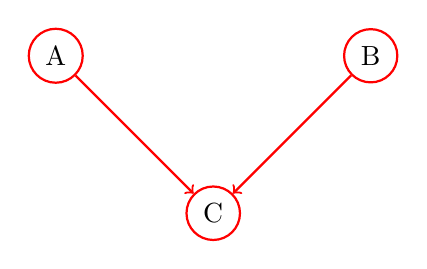
\begin{tikzpicture}[
        node/.style={circle, draw=red, thick, minimum size=18pt},
        arrow/.style={->, red, thick}
    ]
    % Nodes
    \node[node] (A) at (-2, 1) {A};
    \node[node] (B) at (2, 1) {B};
    \node[node] (C) at (0, -1) {C};
    % Edges
    \draw[arrow] (A) -- (C);
    \draw[arrow] (B) -- (C);
    \end{tikzpicture}
    \caption{Example of Bayesian Network structure}
\end{figure}
\begin{itemize}
    \item Gene $A$ and Gene $B$ are independent;
    \item Gene $C$ can be influenced by both Gene $A$ and Gene $B$;
\end{itemize}
\begin{center}
    \begin{minipage}{0.4\textwidth}
        \centering
        \label{tab:cpdGeneA}
        \begin{tabular}{c|c|c}
            Gene &  Value & P(value)\\ 
            \hline
            A & active   & 0.3\\
            A & inactive & 0.7\\
        \end{tabular}
        \captionof{table}{CPD for Gene A}
    \end{minipage}
    \hfill
    \begin{minipage}{0.4\textwidth}
    \centering
        \label{tab:cpdGeneB}
        \begin{tabular}{c|c|c}
            Gene &  Value & P(value)\\ 
            \hline
            B & active   & 0.3\\
            B & inactive & 0.7\\
        \end{tabular}
        \captionof{table}{CPD for Gene B}
    \end{minipage}
\end{center}

\begin{center}
\begin{tabular}{|c|c|cc|cc|}
\hline
 & & \multicolumn{4}{c|}{A} \\
 & & \multicolumn{2}{c|}{active} & \multicolumn{2}{c|}{inactive} \\
\cline{3-6}
 & & \multicolumn{2}{c|}{B} & \multicolumn{2}{c|}{B} \\
 & & active & inactive & active & inactive \\
\hline
\multirow{2}{*}{C}
 & active   & 0.9 & 0.6 & 0.7 & 0.1 \\
 & inactive & 0.1 & 0.4 & 0.3 & 0.9 \\
\hline
\end{tabular}
\captionof{table}{Conditional Probability Table for Gene C}
\end{center}

\subsection{D-separation}
Before introducing the concept of D-separation, we need to better understand the concept of independence and conditional independence.
We will then present the basic structures that can appear in a BN.

\subsubsection{Independence and conditional independence}
We usually say that, two variables $a, b$ are independent (written $a \perp b|\empty$) if:
    \[ P(a, b) = P(a) P(b) \]
\defib{Conditional independence}{
    We say that two variables $a, b$ are conditionally independent given a third variable $c$ (written $a \perp b | c$) if:
    \[ P(a, b | c) = P(a | c) P(b | c) \]
}
Both independence and conditional independence can be verified by applying basic rules of probability.
Instead, BN allow to verify this properties through the concept of D-separation.

\subsubsection{Tail-to-tail connection}
In a tail-to-tail connection, two variables $a$ and $b$ are connected through a common parent variable $c$:
\begin{figure}[H]
\centering
    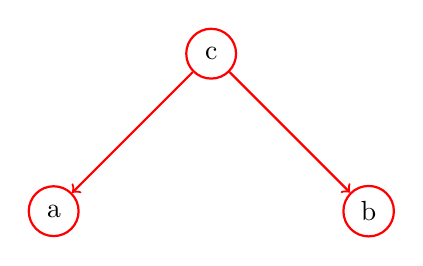
\begin{tikzpicture}[
        node/.style={circle, draw=red, thick, minimum size=18pt},
        arrow/.style={->, red, thick}
    ]
    % Nodes
    \node[node] (C) at (0, 1) {c};
    \node[node] (A) at (-2, -1) {a};
    \node[node] (B) at (2, -1) {b};
    % Edges
    \draw[arrow] (C) -- (A);
    \draw[arrow] (C) -- (B);
    \end{tikzpicture}
    \caption{Tail-to-tail connection}
\end{figure}
The joint distribution can be expressed as:
\begin{equation}
    P(a, b, c) = P(a | c) P(b| c) P(c)
\end{equation}
Given this, we want to understand the independency relationships between $a$ and $b$.
\begin{itemize}
    \item a
\end{itemize}


